\subsection{Les systèmes}
\subsubsection{Définition}

Système = motif + texte\\
motif = rythmes coordonnés joués avec 2 ou 3 membres en boucle\\
texte = rythme irrégulier joué avec un seul membre sur le motif.\\

Quatre systèmes standards :
\begin{itemize}
	\item binaire
	\item ternaire (shuffle, afro, rock)
	\item jazz
	\item afro-cubain
\end{itemize}

\subsubsection{Utilité}
\begin{itemize}
	\item Séparation des voix
	\item Définir une métrique
	\item Conditionner des règles spécifiques de réécriture
\end{itemize}
\ \\
Créer un ensemble de systèmes :
\begin{itemize}
	\item 4/4 binaire FAIT
	\item jazz vs ternaire(12/8) EN COURS…
	\item afro-cubain
	\item Tout transcrire avec lilypond et en arbres d’analyse syntaxique.
	\item Créer les arbres de voix séparées.
	\item Écrire les règles de réécriture.
	\item Créer les arbres de voix séparées simplifiés (rewriting).\\	
\end{itemize}

Pour la \textbf{séparation des voix} et la \textbf{définition des métriques}, nous nous intéresserons principalement à la partie \textit{motif} des systèmes qui seront présentés. La partie \textit{texte} nous intéressera plus pour les \textbf{combinaisons de réécritures}.
\newpage
\subsubsection{Pour la séparation des voix}
\textbf{Motif 4-4 binaire}\\\\
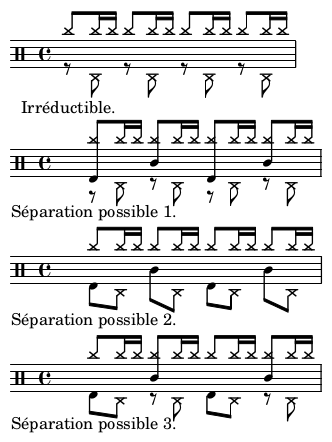
\includegraphics[height=60mm, width=40mm]{z_images/1_description_notation/separation/1_separation_4-4_binaire.png}\\\\
Ici, le système est construit sur un modèle rock en 4/4 : after-beat sur les 2 et 4 avec un choix de répartition des cymbales type fast-jazz. Le système est constitué par défaut du motif ride/ch-pf/cc et d’un texte joué à la grosse-caisse. La troisième séparation proposée est privilégiée car elle répartit selon 2 voix, une voix pour les mains (ride + cc) et une voix pour les pieds (ch-pf + gc). Ce choix paraît plus équilibré car deux instruments sont utilisés par voix et plus logique pour le lecteur puisque les mains sont en haut et les pieds en bas.\\
%D’autres choix d’écriture auraient été possibles :
%\begin{itemize}
%	\item Toutes les hampes en haut ;
%	\item Combinaison motif 1 et 2 en donnant 2 directions aux hampes de la cc).\\
%\end{itemize}

\textbf{Motif 4-4 jazz}\\\\
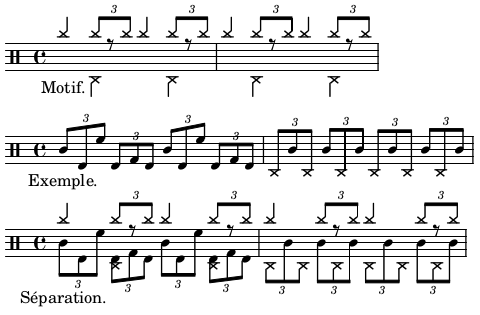
\includegraphics[height=45mm, width=60mm]{z_images/1_description_notation/separation/2_separation_4-4_jazz.png}\\\\
Dans la plupart des méthodes, le charley n’est pas écrit car considéré comme évident en jazz traditionnel. Ce qui facilite grandement l’écriture : la ride et les crash sur la voix du haut et le reste sur la voix du bas. Ici, le partie prit et de tout écrire. Dans l’exemple ci-dessus, les mesures 1 et 2 combinées avec le \textit{motif} de la première ligne, sont des cas typiques de la batterie jazz. Tout mettre sur la voix haute serait surchargé. De plus, la grosse caisse entre très souvent dans le flot des combinaisons de toms et de caisse claire et son écriture séparée serait inutilement compliquée et peu intuitive pour le lecteur. Le choix de séparation sera donc de laisser les cymbales en haut et toms, caisse-claire, grosse-caisse et pédale de charley en bas.
\newpage

\textbf{Système 4-4 afro-cubain}\\\\
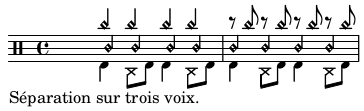
\includegraphics[height=25mm, width=80mm]{z_images/1_description_notation/separation/3_separation_afro-cubain.png}\\\\

\subsubsection{Pour la reconnaissance de la métrique}
\textit{\textbf{12/8 vs 4/4 ternaire}}\\\\
\textbf{Motif 12/8}\\\\
%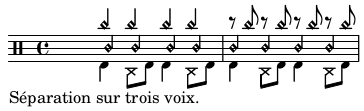
\includegraphics[height=30mm, width=100mm]{z_images/1_description_notation/separation/separation_2.png}\\\\

\subsubsection{Pour les règles de réécriture}
Les textes qui accompagnent les motifs étayent toutes les combinaisons d’un systèmes. 
\newpage

\subsubsection{Construction des systèmes pour les expérimentations}















